\section{zadanie 2}
Zadanie polegało na sprawdzeniu jak programy do wizualizacji funkcji radzą sobie z przedstawieniem funckcji \(f(x) = e^x ln(1+e^{-x})\) oraz policzenie granicy \[\lim_{x \to \infty} f(x) = 1\] 

\subsection{Wnioski:}
Do narysowanie wskazanej funkcji użyłem webowych aplikacji \href{https://www.geogebra.org/calculator}{GeoGebra} i \href{https://mathsolver.microsoft.com/pl}{Microsoft Math Solver}
\begin{figure}[h]
  \centering
  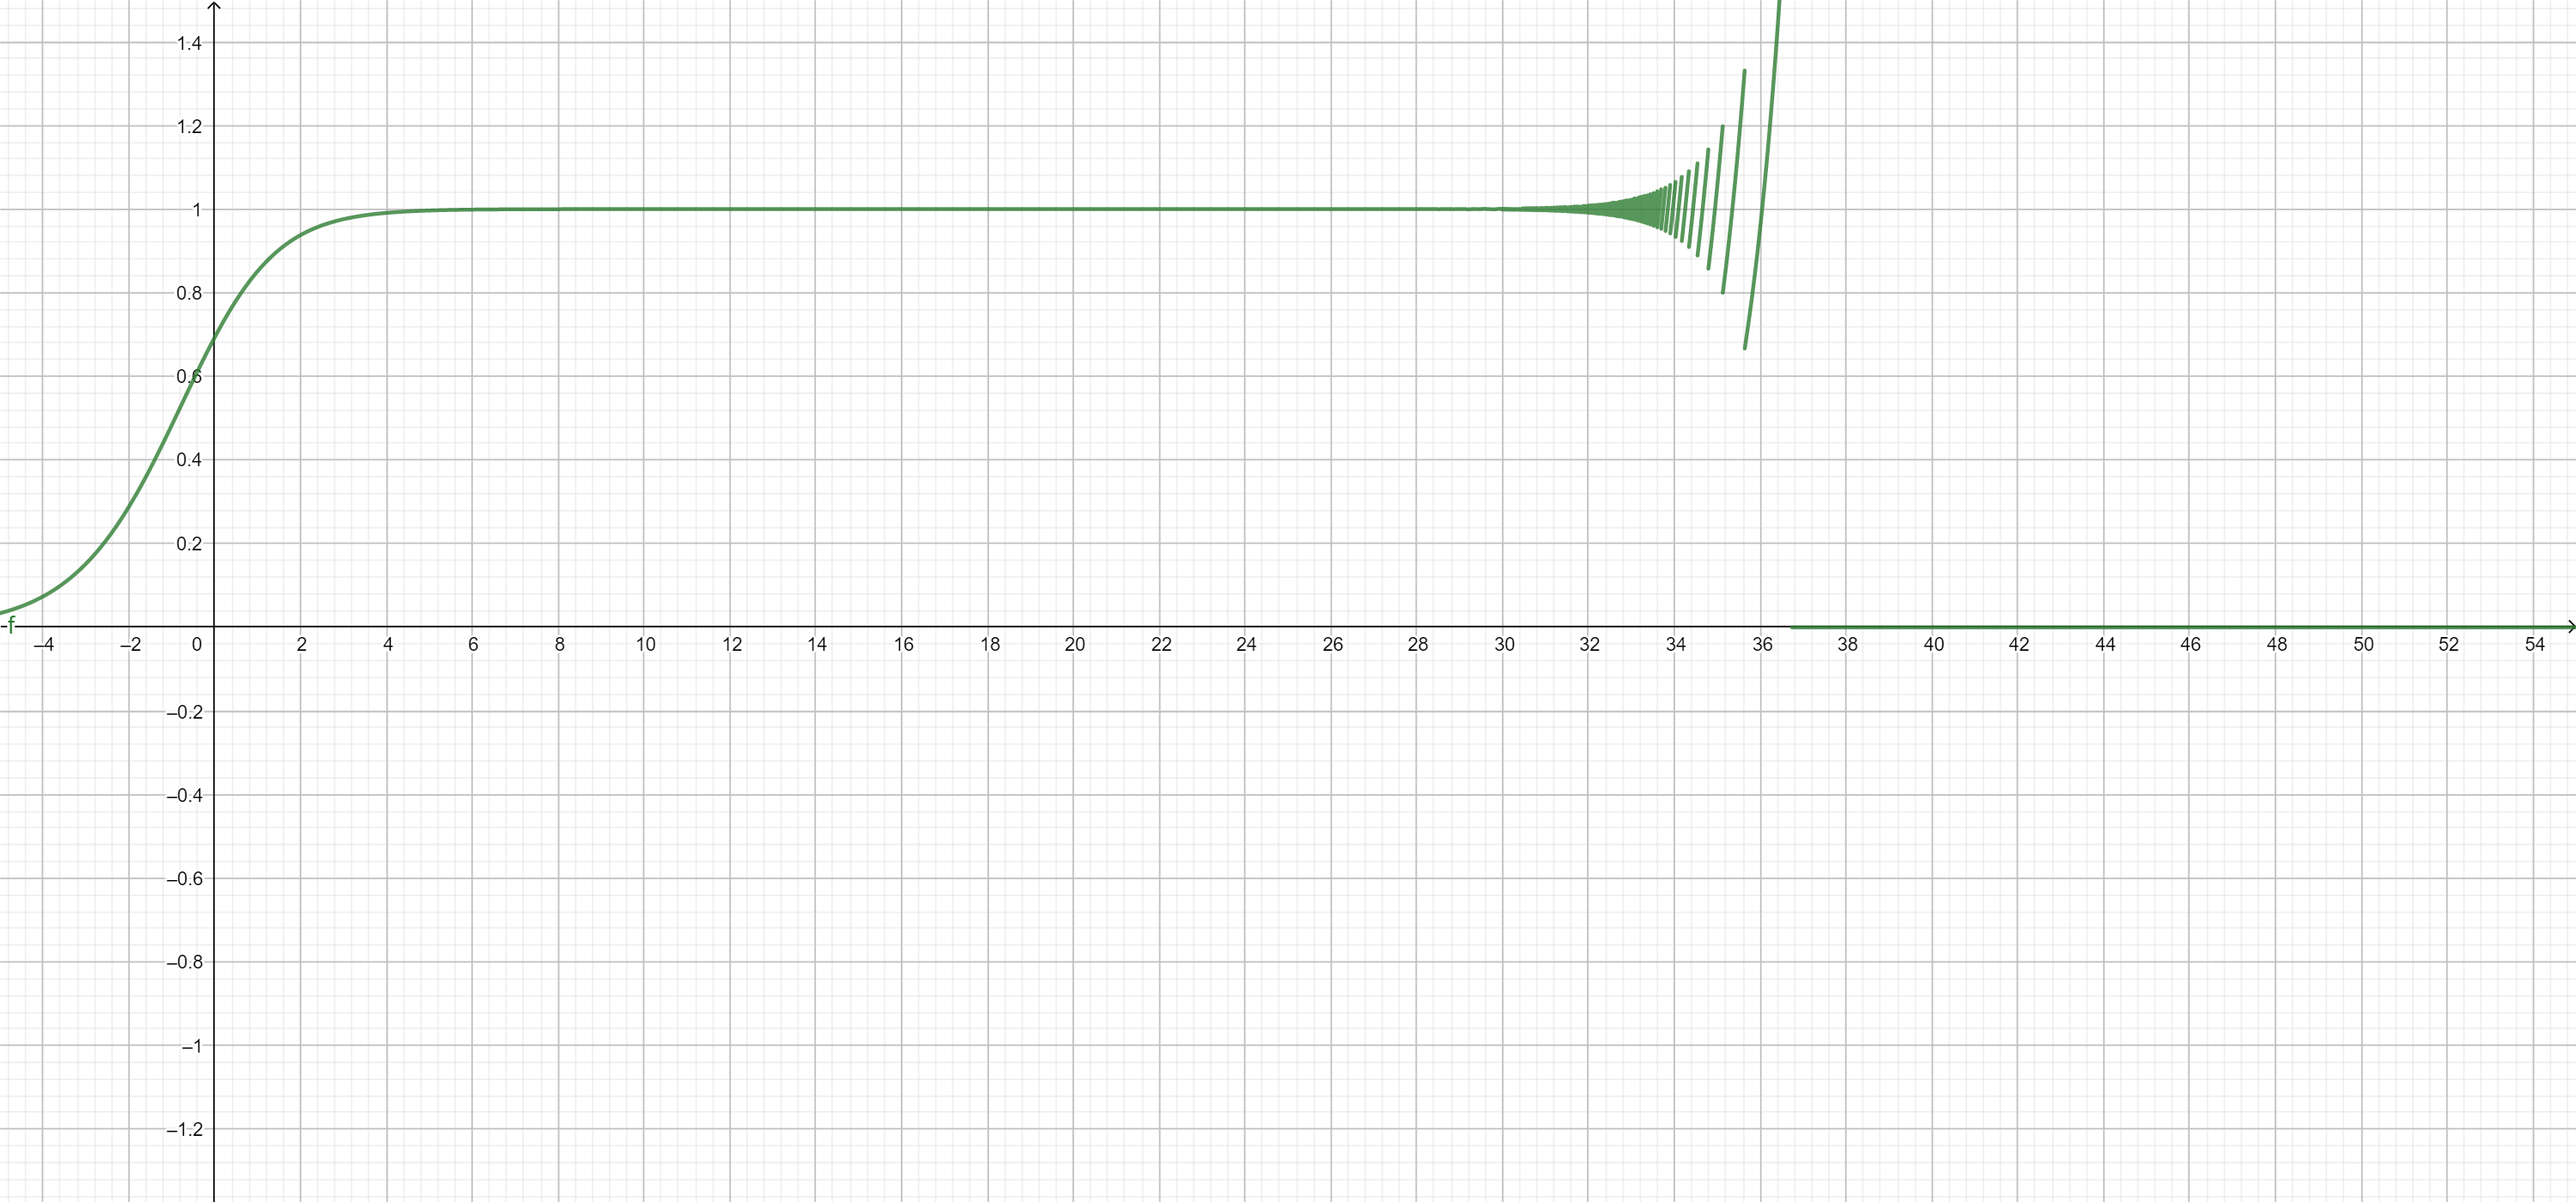
\includegraphics[width=0.75\textwidth]{geogebra.org.png}
  \caption{wykres z GeoGebra}
  \label{fig:geogebra}
\end{figure}
\begin{figure}[h]
  \centering
  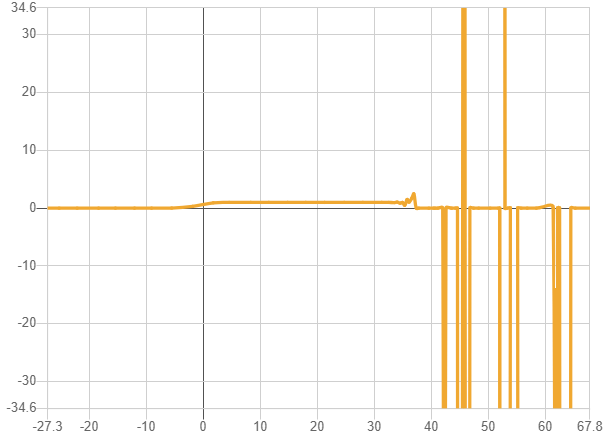
\includegraphics[width=0.75\textwidth]{mathsolver.microsoft.com.png}
  \caption{wykres z Microsoft Math Solver}
  \label{fig:microsoftmathsolver}
\end{figure}

Oba programy rysują błędne wykresy. Wynika to z faktu, że \(e^x\) rośnie wykładniczo, a \(ln(1+e^{-x}) \to 0\), czyli mnożona jest bardzo duża i bardzo mała liczba. Dysponyjemy arytmetyką o skończonej precyzji przez co mantysa traci na precyzji. Przy \(x \approx 35\) wykresy stają się niewiarygodne.
